\PassOptionsToPackage{unicode=true}{hyperref} % options for packages loaded elsewhere
\PassOptionsToPackage{hyphens}{url}
%
\documentclass[ignorenonframetext,]{beamer}
\usepackage{pgfpages}
\setbeamertemplate{caption}[numbered]
\setbeamertemplate{caption label separator}{: }
\setbeamercolor{caption name}{fg=normal text.fg}
\beamertemplatenavigationsymbolsempty
% Prevent slide breaks in the middle of a paragraph:
\widowpenalties 1 10000
\raggedbottom
\setbeamertemplate{part page}{
\centering
\begin{beamercolorbox}[sep=16pt,center]{part title}
  \usebeamerfont{part title}\insertpart\par
\end{beamercolorbox}
}
\setbeamertemplate{section page}{
\centering
\begin{beamercolorbox}[sep=12pt,center]{part title}
  \usebeamerfont{section title}\insertsection\par
\end{beamercolorbox}
}
\setbeamertemplate{subsection page}{
\centering
\begin{beamercolorbox}[sep=8pt,center]{part title}
  \usebeamerfont{subsection title}\insertsubsection\par
\end{beamercolorbox}
}
\AtBeginPart{
  \frame{\partpage}
}
\AtBeginSection{
  \ifbibliography
  \else
    \frame{\sectionpage}
  \fi
}
\AtBeginSubsection{
  \frame{\subsectionpage}
}
\usepackage{lmodern}
\usepackage{amssymb,amsmath}
\usepackage{ifxetex,ifluatex}
\usepackage{fixltx2e} % provides \textsubscript
\ifnum 0\ifxetex 1\fi\ifluatex 1\fi=0 % if pdftex
  \usepackage[T1]{fontenc}
  \usepackage[utf8]{inputenc}
  \usepackage{textcomp} % provides euro and other symbols
\else % if luatex or xelatex
  \usepackage{unicode-math}
  \defaultfontfeatures{Ligatures=TeX,Scale=MatchLowercase}
\fi
% use upquote if available, for straight quotes in verbatim environments
\IfFileExists{upquote.sty}{\usepackage{upquote}}{}
% use microtype if available
\IfFileExists{microtype.sty}{%
\usepackage[]{microtype}
\UseMicrotypeSet[protrusion]{basicmath} % disable protrusion for tt fonts
}{}
\IfFileExists{parskip.sty}{%
\usepackage{parskip}
}{% else
\setlength{\parindent}{0pt}
\setlength{\parskip}{6pt plus 2pt minus 1pt}
}
\usepackage{hyperref}
\hypersetup{
            pdftitle={Math156 Final Project Neural Network Report},
            pdfauthor={Group 5},
            pdfborder={0 0 0},
            breaklinks=true}
\urlstyle{same}  % don't use monospace font for urls
\newif\ifbibliography
\usepackage{color}
\usepackage{fancyvrb}
\newcommand{\VerbBar}{|}
\newcommand{\VERB}{\Verb[commandchars=\\\{\}]}
\DefineVerbatimEnvironment{Highlighting}{Verbatim}{commandchars=\\\{\}}
% Add ',fontsize=\small' for more characters per line
\usepackage{framed}
\definecolor{shadecolor}{RGB}{248,248,248}
\newenvironment{Shaded}{\begin{snugshade}}{\end{snugshade}}
\newcommand{\AlertTok}[1]{\textcolor[rgb]{0.94,0.16,0.16}{#1}}
\newcommand{\AnnotationTok}[1]{\textcolor[rgb]{0.56,0.35,0.01}{\textbf{\textit{#1}}}}
\newcommand{\AttributeTok}[1]{\textcolor[rgb]{0.77,0.63,0.00}{#1}}
\newcommand{\BaseNTok}[1]{\textcolor[rgb]{0.00,0.00,0.81}{#1}}
\newcommand{\BuiltInTok}[1]{#1}
\newcommand{\CharTok}[1]{\textcolor[rgb]{0.31,0.60,0.02}{#1}}
\newcommand{\CommentTok}[1]{\textcolor[rgb]{0.56,0.35,0.01}{\textit{#1}}}
\newcommand{\CommentVarTok}[1]{\textcolor[rgb]{0.56,0.35,0.01}{\textbf{\textit{#1}}}}
\newcommand{\ConstantTok}[1]{\textcolor[rgb]{0.00,0.00,0.00}{#1}}
\newcommand{\ControlFlowTok}[1]{\textcolor[rgb]{0.13,0.29,0.53}{\textbf{#1}}}
\newcommand{\DataTypeTok}[1]{\textcolor[rgb]{0.13,0.29,0.53}{#1}}
\newcommand{\DecValTok}[1]{\textcolor[rgb]{0.00,0.00,0.81}{#1}}
\newcommand{\DocumentationTok}[1]{\textcolor[rgb]{0.56,0.35,0.01}{\textbf{\textit{#1}}}}
\newcommand{\ErrorTok}[1]{\textcolor[rgb]{0.64,0.00,0.00}{\textbf{#1}}}
\newcommand{\ExtensionTok}[1]{#1}
\newcommand{\FloatTok}[1]{\textcolor[rgb]{0.00,0.00,0.81}{#1}}
\newcommand{\FunctionTok}[1]{\textcolor[rgb]{0.00,0.00,0.00}{#1}}
\newcommand{\ImportTok}[1]{#1}
\newcommand{\InformationTok}[1]{\textcolor[rgb]{0.56,0.35,0.01}{\textbf{\textit{#1}}}}
\newcommand{\KeywordTok}[1]{\textcolor[rgb]{0.13,0.29,0.53}{\textbf{#1}}}
\newcommand{\NormalTok}[1]{#1}
\newcommand{\OperatorTok}[1]{\textcolor[rgb]{0.81,0.36,0.00}{\textbf{#1}}}
\newcommand{\OtherTok}[1]{\textcolor[rgb]{0.56,0.35,0.01}{#1}}
\newcommand{\PreprocessorTok}[1]{\textcolor[rgb]{0.56,0.35,0.01}{\textit{#1}}}
\newcommand{\RegionMarkerTok}[1]{#1}
\newcommand{\SpecialCharTok}[1]{\textcolor[rgb]{0.00,0.00,0.00}{#1}}
\newcommand{\SpecialStringTok}[1]{\textcolor[rgb]{0.31,0.60,0.02}{#1}}
\newcommand{\StringTok}[1]{\textcolor[rgb]{0.31,0.60,0.02}{#1}}
\newcommand{\VariableTok}[1]{\textcolor[rgb]{0.00,0.00,0.00}{#1}}
\newcommand{\VerbatimStringTok}[1]{\textcolor[rgb]{0.31,0.60,0.02}{#1}}
\newcommand{\WarningTok}[1]{\textcolor[rgb]{0.56,0.35,0.01}{\textbf{\textit{#1}}}}
\usepackage{graphicx,grffile}
\makeatletter
\def\maxwidth{\ifdim\Gin@nat@width>\linewidth\linewidth\else\Gin@nat@width\fi}
\def\maxheight{\ifdim\Gin@nat@height>\textheight\textheight\else\Gin@nat@height\fi}
\makeatother
% Scale images if necessary, so that they will not overflow the page
% margins by default, and it is still possible to overwrite the defaults
% using explicit options in \includegraphics[width, height, ...]{}
\setkeys{Gin}{width=\maxwidth,height=\maxheight,keepaspectratio}
\setlength{\emergencystretch}{3em}  % prevent overfull lines
\providecommand{\tightlist}{%
  \setlength{\itemsep}{0pt}\setlength{\parskip}{0pt}}
\setcounter{secnumdepth}{0}

% set default figure placement to htbp
\makeatletter
\def\fps@figure{htbp}
\makeatother


\title{Math156 Final Project Neural Network Report}
\author{Group 5}
\date{7/22/2020}

\begin{document}
\frame{\titlepage}

\begin{frame}[fragile]{PART I. Loading data and Define helper functions}
\protect\hypertarget{part-i.-loading-data-and-define-helper-functions}{}

\begin{Shaded}
\begin{Highlighting}[]
\NormalTok{Vdata <-}\StringTok{ }\KeywordTok{read.csv}\NormalTok{(}\StringTok{"../data/videogames.csv"}\NormalTok{)}
\CommentTok{#Vdata <- Vdata[as.numeric(as.character(Vdata$Year_of_Release)) > 2009, ] # only game after 2010}
\NormalTok{Vdata <-}\StringTok{ }\NormalTok{Vdata[(}\OperatorTok{!}\KeywordTok{is.na}\NormalTok{(Vdata}\OperatorTok{$}\NormalTok{Critic_Score)),] }\CommentTok{# remove missing values}

\NormalTok{Anova_test <-}\StringTok{ }\ControlFlowTok{function}\NormalTok{(classifier, }\DataTypeTok{data =}\NormalTok{ Vdata) \{}
  \KeywordTok{summary}\NormalTok{(}\KeywordTok{aov}\NormalTok{(data}\OperatorTok{$}\NormalTok{Global_Sales }\OperatorTok{~}\StringTok{ }\NormalTok{data[[classifier]]))}
\NormalTok{\}}

\NormalTok{get_freq <-}\StringTok{ }\ControlFlowTok{function}\NormalTok{(x, breaks) \{}
\NormalTok{  len <-}\StringTok{ }\KeywordTok{length}\NormalTok{(breaks)}
\NormalTok{  res <-}\StringTok{ }\KeywordTok{numeric}\NormalTok{(len)}
  \ControlFlowTok{for}\NormalTok{ (i }\ControlFlowTok{in} \KeywordTok{seq_len}\NormalTok{(len)) \{}
\NormalTok{    res[i] <-}\StringTok{ }\KeywordTok{sum}\NormalTok{(breaks[i] }\OperatorTok{<}\StringTok{ }\NormalTok{x }\OperatorTok{&}\StringTok{ }\NormalTok{x }\OperatorTok{<=}\StringTok{ }\NormalTok{breaks[i}\OperatorTok{+}\DecValTok{1}\NormalTok{])}
\NormalTok{  \}}
\NormalTok{  res}
\NormalTok{\}}

\NormalTok{get_density <-}\StringTok{ }\ControlFlowTok{function}\NormalTok{(x, breaks, by) \{}
\NormalTok{  res <-}\StringTok{ }\KeywordTok{get_freq}\NormalTok{(x, breaks) }\OperatorTok{/}\StringTok{ }\NormalTok{(}\KeywordTok{length}\NormalTok{(x) }\OperatorTok{*}\StringTok{ }\NormalTok{by)}
\NormalTok{  res}
\NormalTok{\}}

\NormalTok{get_density_idx <-}\StringTok{ }\ControlFlowTok{function}\NormalTok{(gs) \{}
  \KeywordTok{ceiling}\NormalTok{(}\DecValTok{20} \OperatorTok{*}\StringTok{ }\NormalTok{gs)}
\NormalTok{\}}

\NormalTok{testclass <-}\StringTok{ }\ControlFlowTok{function}\NormalTok{(classifier, }\DataTypeTok{data=}\NormalTok{Vdata)\{}
\NormalTok{  table <-}\StringTok{ }\KeywordTok{tapply}\NormalTok{(Vdata}\OperatorTok{$}\NormalTok{Global_Sales, Vdata[[classifier]], }\ControlFlowTok{function}\NormalTok{(x)\{x\})}
\NormalTok{  table[[}\DecValTok{1}\NormalTok{]] <-}\StringTok{ }\OtherTok{NULL}
  \KeywordTok{par}\NormalTok{(}\DataTypeTok{mfrow =} \KeywordTok{c}\NormalTok{(}\DecValTok{1}\NormalTok{, }\DecValTok{2}\NormalTok{))}
  \KeywordTok{boxplot}\NormalTok{(table, }\DataTypeTok{las =} \DecValTok{3}\NormalTok{, }\DataTypeTok{cex=}\FloatTok{0.2}\NormalTok{, }\DataTypeTok{pch=}\DecValTok{20}\NormalTok{)}
  \KeywordTok{boxplot}\NormalTok{(table, }\DataTypeTok{ylim=}\KeywordTok{c}\NormalTok{(}\DecValTok{0}\NormalTok{,}\DecValTok{5}\NormalTok{), }\DataTypeTok{las =} \DecValTok{3}\NormalTok{, }\DataTypeTok{cex=}\FloatTok{0.2}\NormalTok{,}\DataTypeTok{pch=}\DecValTok{20}\NormalTok{)}
  \KeywordTok{Anova_test}\NormalTok{(classifier)}
\NormalTok{\}}

\NormalTok{rangef <-}\StringTok{ }\ControlFlowTok{function}\NormalTok{(x, }\DataTypeTok{divider=}\DecValTok{5}\NormalTok{) \{}
\NormalTok{  x }\OperatorTok\StringTok{ }\NormalTok{divider }\OperatorTok{*}\StringTok{ }\NormalTok{divider }\OperatorTok{+}\StringTok{ }\NormalTok{divider}\OperatorTok{/}\DecValTok{2}
\NormalTok{\}}
\end{Highlighting}
\end{Shaded}

\end{frame}

\begin{frame}[fragile]{PART II. Heuristically explore the effect of each
paramemter}
\protect\hypertarget{part-ii.-heuristically-explore-the-effect-of-each-paramemter}{}

\begin{block}{Anova test on Genre}

\includegraphics{preprocess_files/figure-beamer/unnamed-chunk-2-1.pdf}

\begin{verbatim}
##                      Df Sum Sq Mean Sq F value   Pr(>F)    
## data[[classifier]]   11    190  17.294    5.27 2.37e-08 ***
## Residuals          8125  26662   3.281                     
## ---
## Signif. codes:  0 '***' 0.001 '**' 0.01 '*' 0.05 '.' 0.1 ' ' 1
\end{verbatim}

\end{block}

\begin{block}{Avona test on Platform}

\includegraphics{preprocess_files/figure-beamer/unnamed-chunk-3-1.pdf}

\begin{verbatim}
##                      Df Sum Sq Mean Sq F value   Pr(>F)    
## data[[classifier]]   11    190  17.294    5.27 2.37e-08 ***
## Residuals          8125  26662   3.281                     
## ---
## Signif. codes:  0 '***' 0.001 '**' 0.01 '*' 0.05 '.' 0.1 ' ' 1
\end{verbatim}

\end{block}

\begin{block}{Anova test on Publisher}

\includegraphics{preprocess_files/figure-beamer/unnamed-chunk-4-1.pdf}

\begin{verbatim}
##                      Df Sum Sq Mean Sq F value Pr(>F)    
## data[[classifier]]  303   2447   8.077   2.592 <2e-16 ***
## Residuals          7833  24405   3.116                   
## ---
## Signif. codes:  0 '***' 0.001 '**' 0.01 '*' 0.05 '.' 0.1 ' ' 1
\end{verbatim}

\end{block}

\end{frame}

\begin{frame}[fragile]{Plot Global Sale \textasciitilde{} Paramemter}
\protect\hypertarget{plot-global-sale-paramemter}{}

\begin{block}{Critic\_Score defines an upperbound}

\includegraphics{preprocess_files/figure-beamer/unnamed-chunk-5-1.pdf}

\end{block}

\begin{block}{Test multicolineality}

\begin{Shaded}
\begin{Highlighting}[]
\KeywordTok{cor.test}\NormalTok{(}\KeywordTok{as.numeric}\NormalTok{(}\KeywordTok{as.character}\NormalTok{(Vdata}\OperatorTok{$}\NormalTok{User_Score)), Vdata}\OperatorTok{$}\NormalTok{Critic_Score)}
\end{Highlighting}
\end{Shaded}

\begin{verbatim}
## Warning in cor.test(as.numeric(as.character(Vdata$User_Score)),
## Vdata$Critic_Score): NAs introduced by coercion
\end{verbatim}

\begin{verbatim}
## 
##  Pearson's product-moment correlation
## 
## data:  as.numeric(as.character(Vdata$User_Score)) and Vdata$Critic_Score
## t = 59.769, df = 7015, p-value < 2.2e-16
## alternative hypothesis: true correlation is not equal to 0
## 95 percent confidence interval:
##  0.5651609 0.5961733
## sample estimates:
##       cor 
## 0.5808778
\end{verbatim}

\end{block}

\end{frame}

\begin{frame}[fragile]{Focus on Critic score}
\protect\hypertarget{focus-on-critic-score}{}

\begin{block}{Make a box plot for Global Sale \textasciitilde{} Critic
Score}

\begin{Shaded}
\begin{Highlighting}[]
\NormalTok{x <-}\StringTok{ }\KeywordTok{seq}\NormalTok{(}\DecValTok{0}\NormalTok{,}\DecValTok{100}\NormalTok{,}\DataTypeTok{len=}\DecValTok{1000}\NormalTok{)}
\NormalTok{y <-}\StringTok{ }\DecValTok{1}\OperatorTok{/}\DecValTok{1500}\OperatorTok{*}\NormalTok{x}\OperatorTok{^}\DecValTok{2}
\NormalTok{idx <-}\StringTok{ }\NormalTok{Vdata}\OperatorTok{$}\NormalTok{Global_Sales }\OperatorTok{<=}\StringTok{ }\NormalTok{(Vdata}\OperatorTok{$}\NormalTok{Critic_Score)}\OperatorTok{^}\DecValTok{2}\OperatorTok{/}\DecValTok{1500}
\KeywordTok{plot}\NormalTok{((Vdata}\OperatorTok{$}\NormalTok{Critic_Score)[idx],Vdata}\OperatorTok{$}\NormalTok{Global_Sales[idx], }\DataTypeTok{cex=}\FloatTok{0.1}\NormalTok{)}
\KeywordTok{lines}\NormalTok{(x,y,}\DataTypeTok{lty=}\DecValTok{3}\NormalTok{,}\DataTypeTok{col=}\StringTok{"red"}\NormalTok{)}
\end{Highlighting}
\end{Shaded}

\includegraphics{preprocess_files/figure-beamer/unnamed-chunk-7-1.pdf}

\begin{Shaded}
\begin{Highlighting}[]
\KeywordTok{plot}\NormalTok{(}\KeywordTok{factor}\NormalTok{((Vdata}\OperatorTok{$}\NormalTok{Critic_Score)[idx]), }\DataTypeTok{ylim=}\KeywordTok{c}\NormalTok{(}\DecValTok{0}\NormalTok{,}\DecValTok{5}\NormalTok{),Vdata}\OperatorTok{$}\NormalTok{Global_Sales[idx], }\DataTypeTok{cex=}\FloatTok{0.1}\NormalTok{)}
\NormalTok{f <-}\StringTok{ }\DecValTok{1}\OperatorTok{/}\DecValTok{20000000}\OperatorTok{*}\NormalTok{x}\OperatorTok{^}\DecValTok{4}\OperatorTok{+}\DecValTok{1}\OperatorTok{/}\DecValTok{1500000000}\OperatorTok{*}\NormalTok{x}\OperatorTok{^}\DecValTok{5}\FloatTok{+0.2}
\NormalTok{t <-}\StringTok{ }\DecValTok{1}\OperatorTok{/}\DecValTok{50000000}\OperatorTok{*}\NormalTok{x}\OperatorTok{^}\DecValTok{4}
\NormalTok{m <-}\StringTok{ }\DecValTok{1}\OperatorTok{/}\DecValTok{80000000}\OperatorTok{*}\NormalTok{x}\OperatorTok{^}\DecValTok{4}\OperatorTok{+}\DecValTok{1}\OperatorTok{/}\DecValTok{2000000000}\OperatorTok{*}\NormalTok{x}\OperatorTok{^}\DecValTok{5}\FloatTok{+0.1}
\KeywordTok{lines}\NormalTok{(x,f,}\DataTypeTok{lty=}\DecValTok{2}\NormalTok{,}\DataTypeTok{col=}\StringTok{"red"}\NormalTok{)}
\KeywordTok{lines}\NormalTok{(x,t,}\DataTypeTok{lty=}\DecValTok{2}\NormalTok{,}\DataTypeTok{col=}\StringTok{"blue"}\NormalTok{)}
\KeywordTok{lines}\NormalTok{(x,m,}\DataTypeTok{lty=}\DecValTok{2}\NormalTok{,}\DataTypeTok{col=}\StringTok{"green"}\NormalTok{)}
\end{Highlighting}
\end{Shaded}

\includegraphics{preprocess_files/figure-beamer/unnamed-chunk-7-2.pdf}

\end{block}

\begin{block}{Group the boxplot by range of 5}

\begin{Shaded}
\begin{Highlighting}[]
\NormalTok{Vdata <-}\StringTok{ }\NormalTok{Vdata[idx, ]}
\NormalTok{Vdata <-}\StringTok{ }\NormalTok{Vdata[Vdata}\OperatorTok{$}\NormalTok{Global_Sales }\OperatorTok{<=}\StringTok{ }\DecValTok{4}\NormalTok{, ]}
\NormalTok{ran <-}\StringTok{ }\KeywordTok{rangef}\NormalTok{(Vdata}\OperatorTok{$}\NormalTok{Critic_Score)}
\KeywordTok{plot}\NormalTok{(}\KeywordTok{factor}\NormalTok{(ran), }\DataTypeTok{ylim=}\KeywordTok{c}\NormalTok{(}\DecValTok{0}\NormalTok{,}\DecValTok{5}\NormalTok{),Vdata}\OperatorTok{$}\NormalTok{Global_Sales, }\DataTypeTok{cex=}\FloatTok{0.1}\NormalTok{)}
\end{Highlighting}
\end{Shaded}

\includegraphics{preprocess_files/figure-beamer/unnamed-chunk-8-1.pdf}

\begin{Shaded}
\begin{Highlighting}[]
\ControlFlowTok{for}\NormalTok{ (i }\ControlFlowTok{in} \KeywordTok{seq}\NormalTok{(}\DecValTok{11}\NormalTok{)) \{}
  \KeywordTok{hist}\NormalTok{(Vdata}\OperatorTok{$}\NormalTok{Global_Sales[ran }\OperatorTok{==}\StringTok{ }\NormalTok{(}\FloatTok{32.5}\OperatorTok{+}\DecValTok{5}\OperatorTok{*}\NormalTok{i)], }\DataTypeTok{breaks=}\KeywordTok{seq}\NormalTok{(}\DecValTok{0}\NormalTok{,}\DecValTok{6}\NormalTok{,}\DataTypeTok{by=}\FloatTok{0.05}\NormalTok{), }\DataTypeTok{main =}
         \KeywordTok{paste}\NormalTok{(}\StringTok{"Sale for Critic Score within "}\NormalTok{, }\StringTok{"["}\NormalTok{,}\KeywordTok{as.character}\NormalTok{(}\FloatTok{32.5}\OperatorTok{+}\DecValTok{5}\OperatorTok{*}\NormalTok{i}\FloatTok{-2.5}\NormalTok{), }\StringTok{","}\NormalTok{,}
        \KeywordTok{as.character}\NormalTok{(}\FloatTok{32.5}\OperatorTok{+}\DecValTok{5}\OperatorTok{*}\NormalTok{i}\FloatTok{+2.5}\NormalTok{),}\StringTok{"]"}\NormalTok{), }\DataTypeTok{xlab=}\StringTok{"Global Sale"}\NormalTok{, }\DataTypeTok{probability =} \OtherTok{TRUE}\NormalTok{)}
  \KeywordTok{lines}\NormalTok{(}\KeywordTok{seq}\NormalTok{(}\DecValTok{0}\NormalTok{,}\DecValTok{4}\NormalTok{,}\DataTypeTok{by=}\FloatTok{0.05}\NormalTok{)}\OperatorTok{+}\FloatTok{0.025}\NormalTok{, }\KeywordTok{get_density}\NormalTok{(Vdata}\OperatorTok{$}\NormalTok{Global_Sales[ran }\OperatorTok{==}\StringTok{ }\NormalTok{(}\FloatTok{32.5}\OperatorTok{+}\DecValTok{5}\OperatorTok{*}\NormalTok{i)], }\KeywordTok{seq}\NormalTok{(}\DecValTok{0}\NormalTok{,}\DecValTok{4}\NormalTok{,}\DataTypeTok{by=}\FloatTok{0.05}\NormalTok{), }\FloatTok{0.05}\NormalTok{), }\DataTypeTok{col=}\StringTok{"blue"}\NormalTok{)}
  \KeywordTok{legend}\NormalTok{(}\StringTok{"topright"}\NormalTok{, }\StringTok{"Density Curve"}\NormalTok{, }\DataTypeTok{lwd =} \FloatTok{0.5}\NormalTok{, }\DataTypeTok{col =} \StringTok{"blue"}\NormalTok{)}
\NormalTok{\}}
\end{Highlighting}
\end{Shaded}

\includegraphics{preprocess_files/figure-beamer/unnamed-chunk-8-2.pdf}
\includegraphics{preprocess_files/figure-beamer/unnamed-chunk-8-3.pdf}
\includegraphics{preprocess_files/figure-beamer/unnamed-chunk-8-4.pdf}
\includegraphics{preprocess_files/figure-beamer/unnamed-chunk-8-5.pdf}
\includegraphics{preprocess_files/figure-beamer/unnamed-chunk-8-6.pdf}
\includegraphics{preprocess_files/figure-beamer/unnamed-chunk-8-7.pdf}
\includegraphics{preprocess_files/figure-beamer/unnamed-chunk-8-8.pdf}
\includegraphics{preprocess_files/figure-beamer/unnamed-chunk-8-9.pdf}
\includegraphics{preprocess_files/figure-beamer/unnamed-chunk-8-10.pdf}
\includegraphics{preprocess_files/figure-beamer/unnamed-chunk-8-11.pdf}
\includegraphics{preprocess_files/figure-beamer/unnamed-chunk-8-12.pdf}

\end{block}

\end{frame}

\begin{frame}{Set up of the problem}
\protect\hypertarget{set-up-of-the-problem}{}

\begin{itemize}
\tightlist
\item
  The goal is to approximate the blue density curve given the value of
  Critic Score
\item
  We want to get the distribution density function of Global Sale given
  Critic Score: \[f(sale, critic)\]
\item
  We choose MSE as objective function: \[\sum(f-\hat f)^2\]
\end{itemize}

\end{frame}

\begin{frame}[fragile]{Clear up the dataframe and save it to csv file}
\protect\hypertarget{clear-up-the-dataframe-and-save-it-to-csv-file}{}

\begin{Shaded}
\begin{Highlighting}[]
\NormalTok{ran <-}\StringTok{ }\KeywordTok{rangef}\NormalTok{(Vdata}\OperatorTok{$}\NormalTok{Critic_Score)}
\NormalTok{dataf <-}\StringTok{ }\KeywordTok{data.frame}\NormalTok{(}\StringTok{"Global_Sale"}\NormalTok{ =}\StringTok{ }\KeywordTok{numeric}\NormalTok{(}\DecValTok{0}\NormalTok{), }\StringTok{"Critic_Score"}\NormalTok{ =}\StringTok{ }\KeywordTok{numeric}\NormalTok{(}\DecValTok{0}\NormalTok{), }\StringTok{"Density"}\NormalTok{ =}\StringTok{ }\KeywordTok{numeric}\NormalTok{(}\DecValTok{0}\NormalTok{))}
\ControlFlowTok{for}\NormalTok{ (i }\ControlFlowTok{in} \KeywordTok{seq}\NormalTok{(}\DecValTok{11}\NormalTok{)) \{}
\NormalTok{  gs <-}\StringTok{ }\NormalTok{Vdata}\OperatorTok{$}\NormalTok{Global_Sales[ran }\OperatorTok{==}\StringTok{ }\NormalTok{(}\FloatTok{32.5}\OperatorTok{+}\DecValTok{5}\OperatorTok{*}\NormalTok{i)]}
\NormalTok{  cs <-}\StringTok{ }\NormalTok{Vdata}\OperatorTok{$}\NormalTok{Critic_Score[ran }\OperatorTok{==}\StringTok{ }\NormalTok{(}\FloatTok{32.5}\OperatorTok{+}\DecValTok{5}\OperatorTok{*}\NormalTok{i)]}
\NormalTok{  ccount <-}\StringTok{ }\KeywordTok{log10}\NormalTok{(Vdata}\OperatorTok{$}\NormalTok{Critic_Count[ran }\OperatorTok{==}\StringTok{ }\NormalTok{(}\FloatTok{32.5}\OperatorTok{+}\DecValTok{5}\OperatorTok{*}\NormalTok{i)])}
\NormalTok{  ds <-}\StringTok{ }\KeywordTok{get_density}\NormalTok{(Vdata}\OperatorTok{$}\NormalTok{Global_Sales[ran }\OperatorTok{==}\StringTok{ }\NormalTok{(}\FloatTok{32.5}\OperatorTok{+}\DecValTok{5}\OperatorTok{*}\NormalTok{i)], }\KeywordTok{seq}\NormalTok{(}\DecValTok{0}\NormalTok{,}\DecValTok{4}\NormalTok{,}\DataTypeTok{by=}\FloatTok{0.05}\NormalTok{), }\FloatTok{0.05}\NormalTok{)}
\NormalTok{  ds_idx <-}\StringTok{ }\KeywordTok{get_density_idx}\NormalTok{(gs)}
\NormalTok{  cs_range <-}\StringTok{ }\FloatTok{32.5}\OperatorTok{+}\DecValTok{5}\OperatorTok{*}\NormalTok{i}
\NormalTok{  ds <-}\StringTok{ }\NormalTok{ds[ds_idx]}
\NormalTok{  dataf <-}\StringTok{ }\KeywordTok{rbind}\NormalTok{(dataf, }\KeywordTok{cbind}\NormalTok{(gs, cs_range,ccount, cs,ds))}
\NormalTok{\}}
\CommentTok{# write.csv(dataf, "CS_GL_FQ.csv")}
\end{Highlighting}
\end{Shaded}

\end{frame}

\begin{frame}{Neural Network Setting}
\protect\hypertarget{neural-network-setting}{}

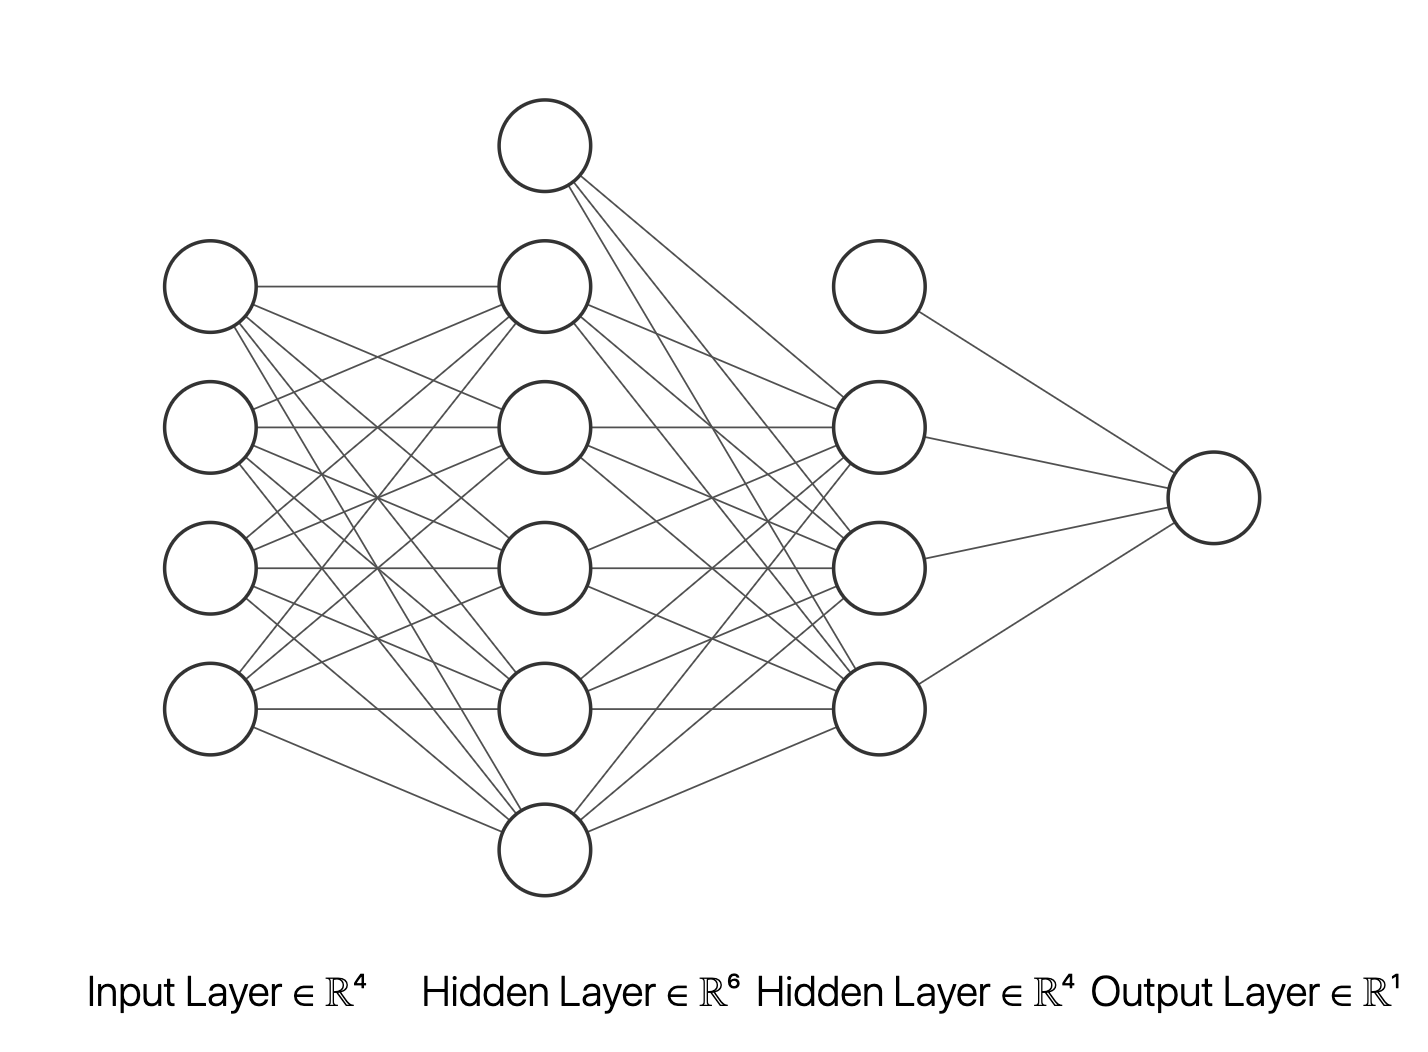
\includegraphics[width=\textwidth,height=3.125in]{nn.png}

\begin{itemize}
\tightlist
\item
  Four input Node: Critic Score, \(log(\text{Critic Count})\), Global
  Sale, Bias
\item
  Activation Function: Exponential Linear Unit(ELU)
  \[\text{elu}(k) = \begin{cases}k  & k>0\\\alpha(e^k-1) & z \leq 0\end{cases}\]
\item
  Optimizer: Adam
\item
  Result: MSE = 0.039741843938827515
\end{itemize}

\end{frame}

\begin{frame}[fragile]{Use elu 4-6-2-1 network Adam
MSE:0.039741843938827515}
\protect\hypertarget{use-elu-4-6-2-1-network-adam-mse0.039741843938827515}{}

\begin{Shaded}
\begin{Highlighting}[]
\NormalTok{Pdata <-}\StringTok{ }\KeywordTok{read.csv}\NormalTok{(}\StringTok{'predictedData.csv'}\NormalTok{)}
\ControlFlowTok{for}\NormalTok{ (i }\ControlFlowTok{in} \KeywordTok{seq}\NormalTok{(}\DecValTok{11}\NormalTok{)) \{}
  \KeywordTok{hist}\NormalTok{(Vdata}\OperatorTok{$}\NormalTok{Global_Sales[ran }\OperatorTok{==}\StringTok{ }\NormalTok{(}\FloatTok{32.5}\OperatorTok{+}\DecValTok{5}\OperatorTok{*}\NormalTok{i)], }\DataTypeTok{breaks=}\KeywordTok{seq}\NormalTok{(}\DecValTok{0}\NormalTok{,}\DecValTok{4}\NormalTok{,}\DataTypeTok{by=}\FloatTok{0.05}\NormalTok{), }\DataTypeTok{main =}
         \KeywordTok{paste}\NormalTok{(}\StringTok{"Sale for Critic Score within "}\NormalTok{, }\StringTok{"["}\NormalTok{,}\KeywordTok{as.character}\NormalTok{(}\FloatTok{32.5}\OperatorTok{+}\DecValTok{5}\OperatorTok{*}\NormalTok{i}\FloatTok{-2.5}\NormalTok{), }\StringTok{","}\NormalTok{,}
        \KeywordTok{as.character}\NormalTok{(}\FloatTok{32.5}\OperatorTok{+}\DecValTok{5}\OperatorTok{*}\NormalTok{i}\FloatTok{+2.5}\NormalTok{),}\StringTok{"]"}\NormalTok{), }\DataTypeTok{xlab=}\StringTok{"Global Sale"}\NormalTok{, }\DataTypeTok{probability =} \OtherTok{TRUE}\NormalTok{)}
  \KeywordTok{lines}\NormalTok{(}\KeywordTok{seq}\NormalTok{(}\DecValTok{0}\NormalTok{,}\DecValTok{4}\NormalTok{,}\DataTypeTok{by=}\FloatTok{0.05}\NormalTok{)}\OperatorTok{+}\FloatTok{0.025}\NormalTok{, }\KeywordTok{get_density}\NormalTok{(Vdata}\OperatorTok{$}\NormalTok{Global_Sales[ran }\OperatorTok{==}\StringTok{ }\NormalTok{(}\FloatTok{32.5}\OperatorTok{+}\DecValTok{5}\OperatorTok{*}\NormalTok{i)], }\KeywordTok{seq}\NormalTok{(}\DecValTok{0}\NormalTok{,}\DecValTok{4}\NormalTok{,}\DataTypeTok{by=}\FloatTok{0.05}\NormalTok{), }\FloatTok{0.05}\NormalTok{), }\DataTypeTok{col=}\StringTok{"blue"}\NormalTok{)}
\NormalTok{  gs <-}\StringTok{ }\NormalTok{Pdata}\OperatorTok{$}\NormalTok{gs[Pdata}\OperatorTok{$}\NormalTok{cs_range }\OperatorTok{==}\StringTok{ }\NormalTok{(}\FloatTok{32.5}\OperatorTok{+}\DecValTok{5}\OperatorTok{*}\NormalTok{i)]}
\NormalTok{  y <-}\StringTok{ }\NormalTok{Pdata[[}\DecValTok{6}\NormalTok{]][Pdata}\OperatorTok{$}\NormalTok{cs_range }\OperatorTok{==}\StringTok{ }\NormalTok{(}\FloatTok{32.5}\OperatorTok{+}\DecValTok{5}\OperatorTok{*}\NormalTok{i)]}
  \KeywordTok{points}\NormalTok{(gs, y, }\DataTypeTok{col=}\StringTok{'red'}\NormalTok{, }\DataTypeTok{pch=}\DecValTok{19}\NormalTok{,}\DataTypeTok{cex=}\FloatTok{0.5}\NormalTok{)}
  \KeywordTok{legend}\NormalTok{(}\StringTok{"topright"}\NormalTok{, }\KeywordTok{c}\NormalTok{(}\StringTok{"Density Curve"}\NormalTok{, }\StringTok{"Predicted By Neural Network"}\NormalTok{), }\DataTypeTok{lwd =} \KeywordTok{c}\NormalTok{(}\FloatTok{0.5}\NormalTok{, }\OtherTok{NA}\NormalTok{), }\DataTypeTok{col =} \KeywordTok{c}\NormalTok{(}\StringTok{"blue"}\NormalTok{, }\StringTok{'red'}\NormalTok{), }\DataTypeTok{pch=}\KeywordTok{c}\NormalTok{(}\OtherTok{NA}\NormalTok{, }\DecValTok{19}\NormalTok{))}
\NormalTok{\}}
\end{Highlighting}
\end{Shaded}

\includegraphics{preprocess_files/figure-beamer/unnamed-chunk-10-1.pdf}
\includegraphics{preprocess_files/figure-beamer/unnamed-chunk-10-2.pdf}
\includegraphics{preprocess_files/figure-beamer/unnamed-chunk-10-3.pdf}
\includegraphics{preprocess_files/figure-beamer/unnamed-chunk-10-4.pdf}
\includegraphics{preprocess_files/figure-beamer/unnamed-chunk-10-5.pdf}
\includegraphics{preprocess_files/figure-beamer/unnamed-chunk-10-6.pdf}
\includegraphics{preprocess_files/figure-beamer/unnamed-chunk-10-7.pdf}
\includegraphics{preprocess_files/figure-beamer/unnamed-chunk-10-8.pdf}
\includegraphics{preprocess_files/figure-beamer/unnamed-chunk-10-9.pdf}
\includegraphics{preprocess_files/figure-beamer/unnamed-chunk-10-10.pdf}
\includegraphics{preprocess_files/figure-beamer/unnamed-chunk-10-11.pdf}

\begin{Shaded}
\begin{Highlighting}[]
\NormalTok{Pdata <-}\StringTok{ }\KeywordTok{read.csv}\NormalTok{(}\StringTok{'predictedData2.csv'}\NormalTok{)}
\ControlFlowTok{for}\NormalTok{ (i }\ControlFlowTok{in} \KeywordTok{seq}\NormalTok{(}\DecValTok{11}\NormalTok{)) \{}
  \KeywordTok{hist}\NormalTok{(Vdata}\OperatorTok{$}\NormalTok{Global_Sales[ran }\OperatorTok{==}\StringTok{ }\NormalTok{(}\FloatTok{32.5}\OperatorTok{+}\DecValTok{5}\OperatorTok{*}\NormalTok{i)], }\DataTypeTok{breaks=}\KeywordTok{seq}\NormalTok{(}\DecValTok{0}\NormalTok{,}\DecValTok{4}\NormalTok{,}\DataTypeTok{by=}\FloatTok{0.05}\NormalTok{), }\DataTypeTok{main =}
         \KeywordTok{paste}\NormalTok{(}\StringTok{"Sale for Critic Score within "}\NormalTok{, }\StringTok{"["}\NormalTok{,}\KeywordTok{as.character}\NormalTok{(}\FloatTok{32.5}\OperatorTok{+}\DecValTok{5}\OperatorTok{*}\NormalTok{i}\FloatTok{-2.5}\NormalTok{), }\StringTok{","}\NormalTok{,}
        \KeywordTok{as.character}\NormalTok{(}\FloatTok{32.5}\OperatorTok{+}\DecValTok{5}\OperatorTok{*}\NormalTok{i}\FloatTok{+2.5}\NormalTok{),}\StringTok{"]"}\NormalTok{), }\DataTypeTok{xlab=}\StringTok{"Global Sale"}\NormalTok{, }\DataTypeTok{probability =} \OtherTok{TRUE}\NormalTok{)}
  \KeywordTok{lines}\NormalTok{(}\KeywordTok{seq}\NormalTok{(}\DecValTok{0}\NormalTok{,}\DecValTok{4}\NormalTok{,}\DataTypeTok{by=}\FloatTok{0.05}\NormalTok{)}\OperatorTok{+}\FloatTok{0.025}\NormalTok{, }\KeywordTok{get_density}\NormalTok{(Vdata}\OperatorTok{$}\NormalTok{Global_Sales[ran }\OperatorTok{==}\StringTok{ }\NormalTok{(}\FloatTok{32.5}\OperatorTok{+}\DecValTok{5}\OperatorTok{*}\NormalTok{i)], }\KeywordTok{seq}\NormalTok{(}\DecValTok{0}\NormalTok{,}\DecValTok{4}\NormalTok{,}\DataTypeTok{by=}\FloatTok{0.05}\NormalTok{), }\FloatTok{0.05}\NormalTok{), }\DataTypeTok{col=}\StringTok{"blue"}\NormalTok{)}
\NormalTok{  gs <-}\StringTok{ }\NormalTok{Pdata}\OperatorTok{$}\NormalTok{gs[Pdata}\OperatorTok{$}\NormalTok{cs_range }\OperatorTok{==}\StringTok{ }\NormalTok{(}\FloatTok{32.5}\OperatorTok{+}\DecValTok{5}\OperatorTok{*}\NormalTok{i)]}
\NormalTok{  y <-}\StringTok{ }\NormalTok{Pdata[[}\DecValTok{6}\NormalTok{]][Pdata}\OperatorTok{$}\NormalTok{cs_range }\OperatorTok{==}\StringTok{ }\NormalTok{(}\FloatTok{32.5}\OperatorTok{+}\DecValTok{5}\OperatorTok{*}\NormalTok{i)]}
  \KeywordTok{points}\NormalTok{(gs, y, }\DataTypeTok{col=}\StringTok{'red'}\NormalTok{, }\DataTypeTok{pch=}\DecValTok{19}\NormalTok{,}\DataTypeTok{cex=}\FloatTok{0.5}\NormalTok{)}
  \KeywordTok{legend}\NormalTok{(}\StringTok{"topright"}\NormalTok{, }\KeywordTok{c}\NormalTok{(}\StringTok{"Density Curve"}\NormalTok{, }\StringTok{"Predicted By Neural Network"}\NormalTok{), }\DataTypeTok{lwd =} \KeywordTok{c}\NormalTok{(}\FloatTok{0.5}\NormalTok{, }\OtherTok{NA}\NormalTok{), }\DataTypeTok{col =} \KeywordTok{c}\NormalTok{(}\StringTok{"blue"}\NormalTok{, }\StringTok{'red'}\NormalTok{), }\DataTypeTok{pch=}\KeywordTok{c}\NormalTok{(}\OtherTok{NA}\NormalTok{, }\DecValTok{19}\NormalTok{))}
\NormalTok{\}}
\end{Highlighting}
\end{Shaded}

\includegraphics{preprocess_files/figure-beamer/unnamed-chunk-11-1.pdf}
\includegraphics{preprocess_files/figure-beamer/unnamed-chunk-11-2.pdf}
\includegraphics{preprocess_files/figure-beamer/unnamed-chunk-11-3.pdf}
\includegraphics{preprocess_files/figure-beamer/unnamed-chunk-11-4.pdf}
\includegraphics{preprocess_files/figure-beamer/unnamed-chunk-11-5.pdf}
\includegraphics{preprocess_files/figure-beamer/unnamed-chunk-11-6.pdf}
\includegraphics{preprocess_files/figure-beamer/unnamed-chunk-11-7.pdf}
\includegraphics{preprocess_files/figure-beamer/unnamed-chunk-11-8.pdf}
\includegraphics{preprocess_files/figure-beamer/unnamed-chunk-11-9.pdf}
\includegraphics{preprocess_files/figure-beamer/unnamed-chunk-11-10.pdf}
\includegraphics{preprocess_files/figure-beamer/unnamed-chunk-11-11.pdf}

\end{frame}

\end{document}
